\documentclass[10pt]{article}
\usepackage[letterpaper,margin=1in]{geometry}
\usepackage[T1]{fontenc}
\usepackage[utf8]{inputenc}
\usepackage{booktabs}
\usepackage{graphicx}
\usepackage{amsmath,amssymb}
\usepackage{xcolor}
\usepackage[hidelinks]{hyperref}
\usepackage{caption}
\usepackage{microtype}
\captionsetup{font=small,labelfont=bf}

% --- convenience macros ---
\newcommand{\rhov}{$\rho$}
\newcommand{\loto}{\textsc{loto}}
\newcommand{\code}[1]{\texttt{#1}}

\title{\bfseries Decodable but Not Usable: What a Frozen Code-LLM Knows About\\
ML-Solution Quality, and Why It Does Not Guide Poor-Compute Search}
\author{[Author(s) --- omitted for review]\\[2pt]\small [Affiliation]}
\date{}

\begin{document}
\maketitle

\begin{abstract}
\noindent
Automated ML-engineering agents search over candidate solutions; a natural way to guide that search cheaply is a \emph{critic} that scores a candidate \emph{before} paying to evaluate it. We ask, under deliberately poor compute---a single consumer GPU, and a base search LLM that is never fine-tuned and reached only through an API---whether such a critic can be read out of the internal representations of a \emph{frozen} code-LLM, and whether it actually helps. On 289 externally-graded solutions from three Kaggle-style tabular competitions we find a sharp dissociation. \textbf{The signal is there}: a linear probe on a frozen code-LLM's mid-layer representation decodes the eventual (expensive) grade \emph{across tasks}, and that signal is independent of the candidate's own cheap self-reported score, independent of code length (the make-or-break confound), low-dimensional (one principal direction recovers ${\sim}70\%$), and reproduced across four code-LLMs from three families. \textbf{But the signal is not usable for control}: it buys \emph{no} budget savings under a fixed evaluation budget (\emph{rank $\neq$ regret}); a deployment \emph{veto} built on it evaporates on real search trees; and the quality direction cannot be causally \emph{steered}---only surface features such as code length steer the model's behaviour. A frozen representation \emph{knows} solution quality without being able to \emph{use} it. \textbf{The one thing it can do is detect failure}: the same probe flags reward-hacking / validation-overfit solutions the self-report is blind to (AUROC 0.63; inside the set the self-report trusts, the self-report is actively \emph{anti}-informative), though modestly. A trained reasoning critic and multi-fidelity screening add nothing at this scale. Under poor compute the lever is \textbf{clean evaluation, not a cleverer critic}---a single-GPU, model-agnostic instantiation of the AIRA\_2 diagnosis, delivered as a set of cheap, adversarial, offline falsification tests.
\end{abstract}

\section{Introduction}
LLM agents that do machine-learning engineering---write, run, and refine ML code against a held-out metric---spend most of their budget \emph{evaluating} candidate solutions, since each evaluation trains and scores a model. A controller that could tell a good candidate from a bad one \emph{before} evaluating it would be valuable: it could rank candidates, prune the budget, or steer generation. The obvious such controller is a \textbf{learned critic}.

Two facts make this hard in our regime. First, \textbf{compute is poor}: one RTX 3090, and a base LLM (DeepSeek) that we deliberately never fine-tune---the method must be \emph{model-agnostic}, so all ``learning'' lives in a light-weight readout, not in the base weights. Second, prior work is sobering: aira-dojo~\cite{airadojo} formalises search \emph{policy} $\times$ \emph{operator} and reports that, with evaluation held fixed, the search policy contributes little; AIRA\_2~\cite{aira2} diagnoses the degradation not as memorisation but as \textbf{evaluation inconsistency / noise}. Our study is a single-GPU instantiation of that diagnosis, and asks the concrete question underneath it: \emph{can a cheap critic, read from a frozen code-LLM, recover the signal a noisy evaluation loses---and does recovering it help the search?}

Our answer is a clean dissociation between \textbf{decodability} and \textbf{usability}, which organises the paper.
\begin{itemize}\itemsep2pt
  \item \textbf{The signal is there (\S\ref{sec:h1}).} Framed as linear probing: the grade is decodable cross-task from a frozen code-LLM's representation, and the signal is \emph{independent of the self-report and of code length}, \emph{low-dimensional}, and \emph{general across model families}.
  \item \textbf{It is not usable for control (\S\ref{sec:notusable}).} The same signal \emph{saves no evaluations} (rank $\neq$ regret), \emph{does not convert} as a deployment veto on real trees, and \emph{cannot be steered} (only surface features steer).
  \item \textbf{The one deployable use is failure detection (\S\ref{sec:detect}).} The probe flags reward-hacking the self-report misses---length-independent, self-report-independent---but modestly.
  \item \textbf{Two more non-levers and two pitfalls (\S\ref{sec:other}--\ref{sec:pitfalls}).} A trained reasoning critic and multi-fidelity screening add nothing; two measurement artifacts we hit could each have produced a false headline.
\end{itemize}
Everything is offline, cheap, and \emph{designed to falsify before you build}: we report medians across seeds with dispersion, never single numbers, and surface the confounds ourselves.

\section{Related work}
\textbf{Search-policy negatives.} aira-dojo~\cite{airadojo} is our target: with evaluation fixed, search policy barely matters. AIRA\_2~\cite{aira2} relocates the cause to evaluation noise and proposes a high-consistency evaluation protocol; \S\ref{sec:notusable}--\ref{sec:other} show that two ``obvious fixes'' on the critic side do \emph{not} rescue the affordable regime.

\textbf{Hidden-state reward models.} ELHSR~\cite{elhsr} learns a reward from a \emph{frozen} LLM's hidden states via a linear head---the same family as our probe---but for \textbf{binary correctness} on cheap-to-verify reasoning, used for best-of-$N$ reranking. We borrow the mechanism; our setting is the \textbf{expensive, scarce, continuous} ML grade, and our contribution is an \textbf{ablation-based independence} argument reranking never needs.

\textbf{Probing code-LLMs.} OPENIA~\cite{openia}, AutoProbe~\cite{autoprobe}, and a contrastive-direction code ranker~\cite{ranker} (which uses the same Qwen2.5-Coder-7B) show a frozen code-LLM's hidden states linearly encode \textbf{binary unit-correctness} against a solution's own tests. We differ on two axes: a \textbf{continuous downstream task grade} rather than pass/fail of one unit, and \textbf{verified independence} from the self-report and code length.

\textbf{Steering \& reward hacking.} Steering code-LLMs~\cite{steer} finds the controllable directions are \emph{language/library}, not quality---which \S\ref{sec:notusable} confirms causally. Reward-hacking detection~\cite{rh1,rh2} under the Goodhart framing~\cite{goodhart} is the frame for \S\ref{sec:detect}.

\section{Setup}
\textbf{Data.} 289 ``cards'' harvested from AIRA\_MCTS searches (base LLM {=} DeepSeek, via a LiteLLM/OpenAI-compatible client) on three tabular competitions: \code{spaceship-titanic} (221 cards; classification), \code{nomad2018-predict-transparent-conductors} (37; regression/RMSLE), \code{tabular-playground-series-may-2022} (31; classification). Each \textbf{card} is a candidate solution carrying the task, the generated code, the cheap early signals the agent saw (self-reported validation score \code{val\_at\_low}, runtime, lineage), and---separately, as the \textbf{label}---an \textbf{external, pristine, medal-normalised grade $y$} computed by held-out code the agent never touches. Cards without an official grade are dropped.

\textbf{Models.} The base search LLM is never fine-tuned. The critic's substrate is a \textbf{frozen} code-LLM used only as a feature extractor: primarily Qwen2.5-Coder-7B-Instruct, plus Qwen2.5-Coder-14B, DeepSeek-Coder-6.7B-Instruct, and CodeLlama-7B-Instruct for the cross-family check (\S\ref{sec:crossfamily}). All loaded in 4-bit; a ridge readout is the only thing ``trained''.

\textbf{Integrity \& fair contract.} Grading is external and pristine; the agent sees scores, never labels; there is \textbf{no LLM-as-judge} anywhere. In every comparison \textbf{only the studied knob varies}---operator set, base LLM, per-task budget, task set, and split are fixed and logged. We pin seeds, dependency versions, and the commit, and write one CSV row per run.

\section{The signal is there: representation probing (H1)}\label{sec:h1}
We ask one question: how much of the eventual (expensive) grade is \emph{linearly decodable} from a frozen code-LLM's representation of the candidate code---and is that information already in the candidate's cheap self-report, or merely a proxy for how much code was written? The frozen model is the \emph{object of study}; a ridge readout is the \emph{measurement instrument} (standard linear probing, cf.\ hidden-state reward models~\cite{elhsr}). We report Spearman \rhov, per-task 5-fold CV within-task (\textbf{intra}) and leave-one-task-out (\textbf{\loto}), 3 seeds, 289 cards (Table~\ref{tab:h1}).

\begin{table}[t]\centering
\caption{Grade decodability (Spearman \rhov) from a frozen Qwen2.5-Coder-7B. The ablated cross-task signal survives, and \emph{rises} under length residualisation, while code length alone does not generalise cross-task.}
\label{tab:h1}
\small
\begin{tabular}{lcc}
\toprule
probe (of 28 layers) / condition & intra \rhov & cross-task \loto{} \rhov \\
\midrule
last layer 28, normal & 0.35 & 0.07 \\
mid layer 21, normal & 0.30 & \textbf{0.18} \\
mid layer 21, self-report ablated & 0.28 & \textbf{0.24} \\
\;\;+ code-length residualised & 0.20 & \textbf{0.30} \\
code-length only (floor) & 0.20 & $-$0.07 \\
\bottomrule
\end{tabular}
\end{table}

\begin{figure}[t]\centering
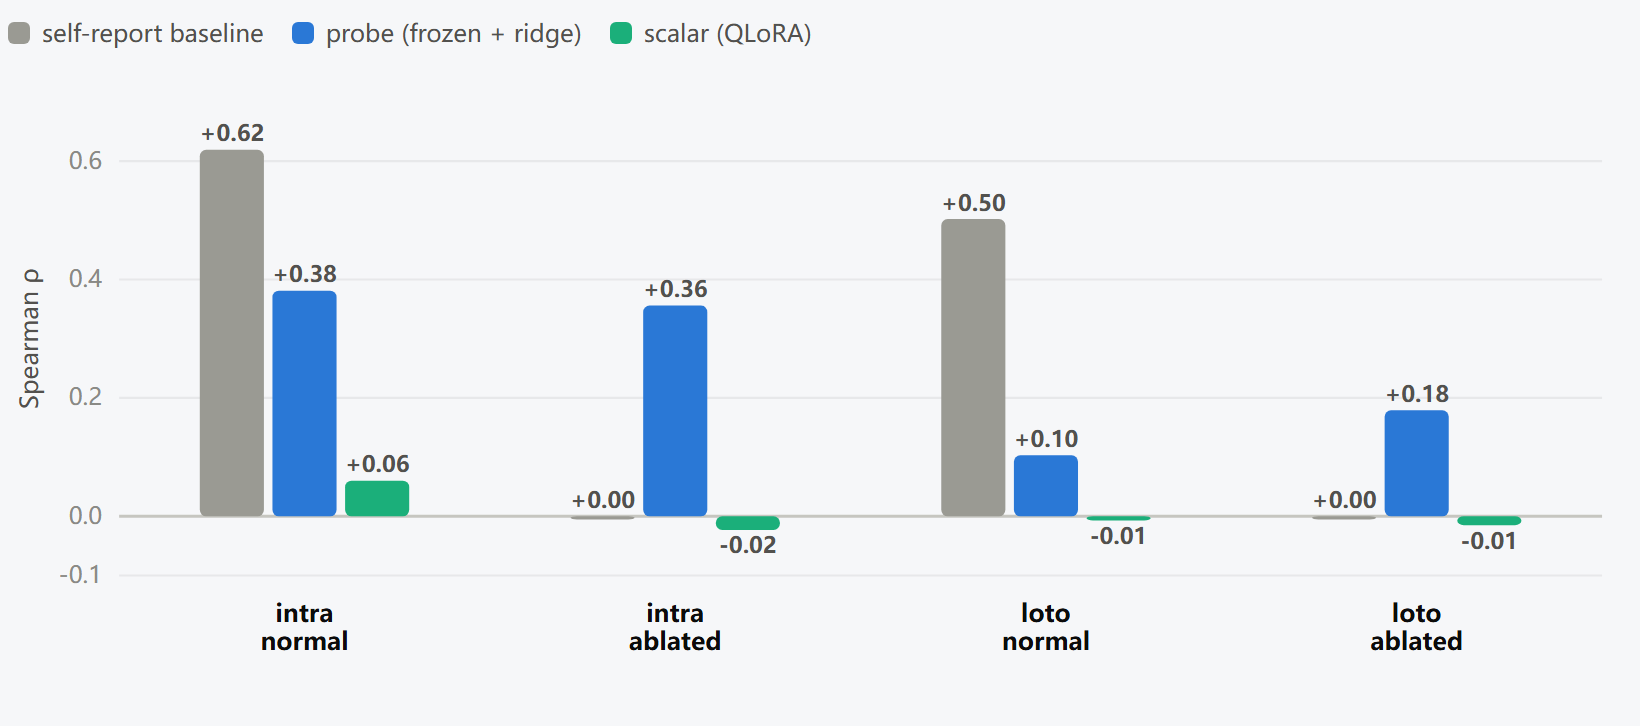
\includegraphics[width=\linewidth]{fig1.png}
\caption{\textbf{H1: the probe carries grade signal independent of the self-report.} Under the self-report ablation the self-report baseline collapses to $0$, but the probe barely drops and \emph{rises} cross-task. The QLoRA scalar head is weak-to-negative throughout.}
\label{fig:h1}
\end{figure}

\textbf{Mid-depth carries the signal best (Fig.~\ref{fig:h1}).} A mid layer (21 of 28) decodes the grade better cross-task than the last-layer default (\loto{} 0.18 vs 0.07), matching the finding that intermediate representations are richest and no fixed final layer is optimal. Concatenating all layers does not help---early layers dilute.

\textbf{It survives ablating the self-report.} Masking the candidate's own \code{val\_at\_low}/curve/parent collapses a self-report-only baseline to exactly $0$, yet the probe barely drops and cross-task \emph{rises} (\loto{} \textbf{0.24}): the representation encodes grade information from the \emph{code itself}, not by echoing the cheap score.

\textbf{It survives controlling for code length---the make-or-break confound.} High probe decodability can be a pure length artifact~\cite{lengtharti}. We residualise every hidden-state dimension against $\log(\text{code length})$ and $\log(\#\text{lines})$, fit on the training fold only. Code length \emph{alone} decodes at \rhov{} 0.20 within-task but $-0.07$ cross-task---\emph{it does not generalise at all}---whereas the residualised probe \emph{holds}, \loto{} rising to \textbf{0.30}. The encoded signal is genuine representational quality, not a length proxy. (Intra carries a mild length confound, so we headline the confound-clean \loto.)

\textbf{The signal is low-dimensional (Fig.~\ref{fig:lowdim}).} Projecting to the top-$k$ PCA components before the ridge, a \emph{single} component already decodes \rhov{} 0.21---${\sim}70\%$ of the full 7{,}169-dim \rhov{} 0.31---and ${\leq}16$ components match it; a single contrastive good-minus-bad direction is weaker (0.10), so the quality signal is the representation's \textbf{top principal variance, not a mean shift}. This mirrors the ``confidence manifold'' result that a frozen LLM's \emph{binary} correctness lives in 3--8 dimensions~\cite{manifold}; our continuous grade behaves the same, so a light ridge---not a deep head---suffices.

\begin{figure}[t]\centering
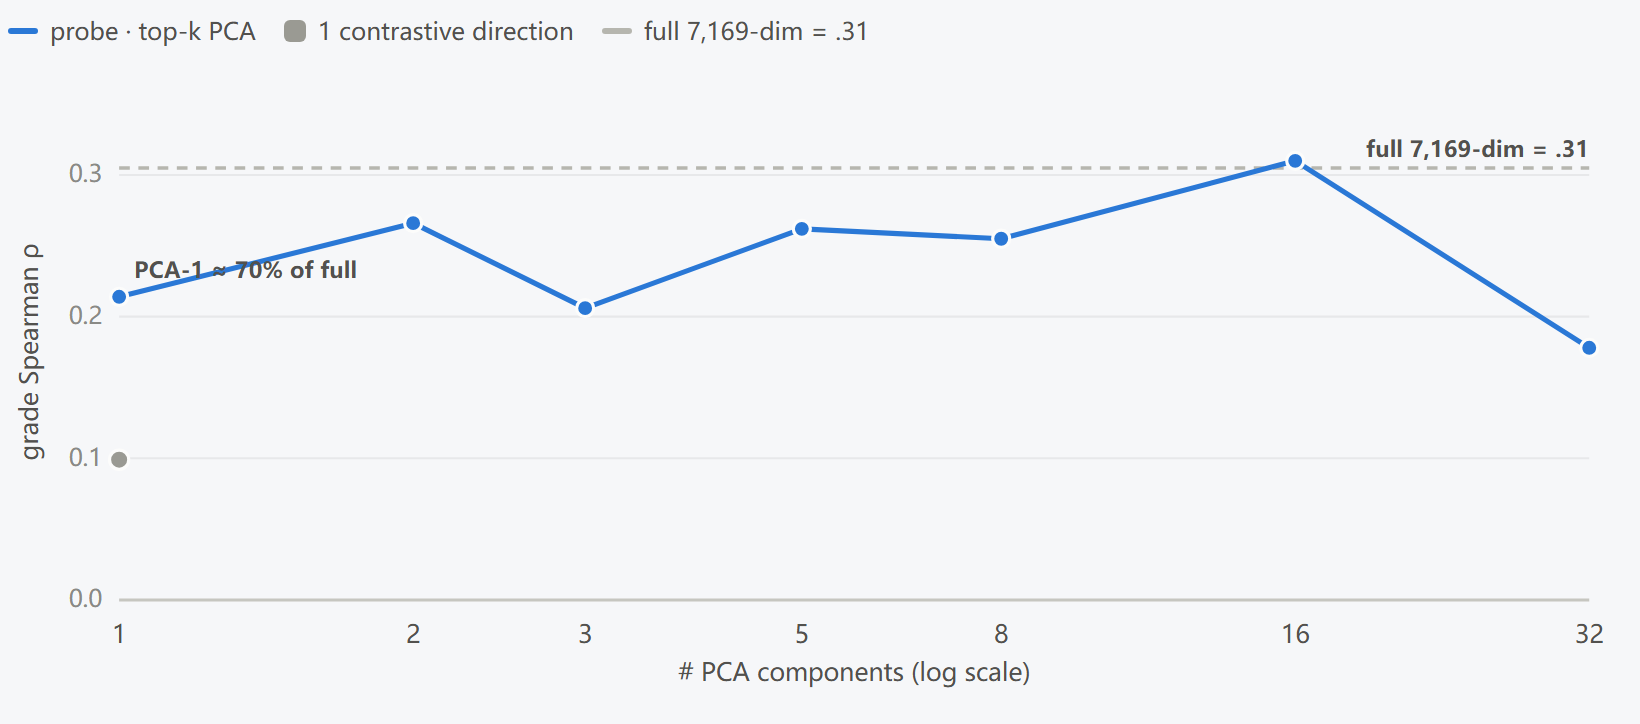
\includegraphics[width=\linewidth]{fig4.png}
\caption{\textbf{The grade signal is low-dimensional.} Grade Spearman vs.\ number of PCA components (per-task 5-fold CV): one component recovers ${\sim}70\%$ of the full-representation signal; ${\leq}16$ match it.}
\label{fig:lowdim}
\end{figure}

\subsection{It replicates across model families}\label{sec:crossfamily}
Running the identical protocol on three further code-LLMs (Fig.~\ref{fig:backbone}), the self-report-ablated, length-residualised cross-task grade signal stays positive in \emph{every} family: \loto{} $=$ \textbf{0.30} (Qwen-Coder-7B) / \textbf{0.23} (Qwen-Coder-14B) / \textbf{0.20} (DeepSeek-Coder-6.7B) / \textbf{0.20} (CodeLlama-7B), all far above the $-0.07$ length floor. Two honest notes: the \emph{best layer} is model-specific (mid-to-late for Qwen; early, ${\sim}25\%$ depth, for DeepSeek/CodeLlama), and \emph{scale does not help} (14B $<$ 7B). What matters is \textbf{that} the backbone is a code-LLM, not its size---the grade signal is a general property of frozen code-LLM representations.

\begin{figure}[t]\centering
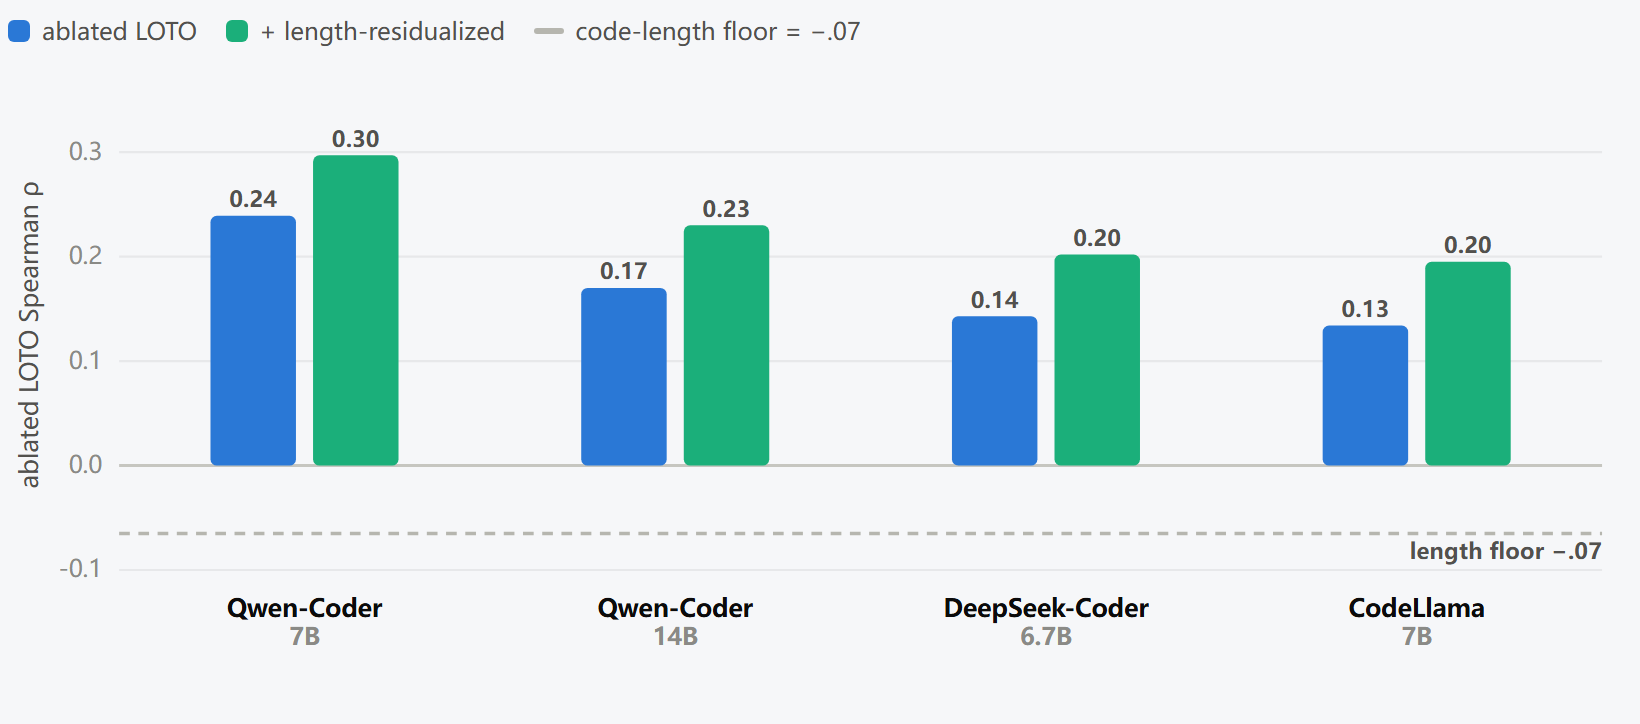
\includegraphics[width=\linewidth]{fig6.png}
\caption{\textbf{H1 replicates across model families---not a Qwen artifact.} Ablated, length-residualised \loto{} grade signal stays positive for four code-LLMs across three families, all above the code-length floor. Scale does not help (14B $<$ 7B).}
\label{fig:backbone}
\end{figure}

\textbf{Novelty.} The closest priors~\cite{openia,autoprobe,ranker} linearly encode \emph{binary unit-correctness} from a frozen code-LLM. We are distinct on two axes no prior makes: a \textbf{continuous eventual task grade}, and \textbf{ablation-verified independence} from both the self-report and code length, general across families. A QLoRA \code{scalar} critic is weak-to-negative at this data scale; H1 rests entirely on the frozen probe---the contribution is \emph{what the representation encodes}, not a trained model.

\section{\dots but the signal is not usable for control}\label{sec:notusable}
The rest of the critic story is one through-line: the decodable signal cannot be turned into a search benefit. Three mechanisms, three negatives.

\subsection{It buys no budget savings (rank $\neq$ regret)}
Under a fixed budget of $K$ expensive evaluations, define $\mathrm{regret}(K){=}\text{oracle}-\text{best-recovered}$. On the one task with real discrimination room (tps-may, dispersed grades; Fig.~\ref{fig:regret}):

\begin{table}[h]\centering\small
\begin{tabular}{lccc}
\toprule
$K{=}3$ & critic (probe) & proxy (self-report) & random \\
\midrule
intra & 0.215 & \textbf{0.000} & 0.171 \\
\loto{} & 0.292 & \textbf{0.000} & 0.227 \\
\bottomrule
\end{tabular}
\end{table}

The \textbf{free self-report proxy is optimal} (it picks the budget's best), while the probe ${\approx}$ random and cross-task \emph{worse} than random. \textbf{No regime makes the probe the right selector}---its ${+}0.4$ rank advantage does not translate into savings. This is the NAS \emph{rank $\neq$ regret} warning.

\begin{figure}[t]\centering
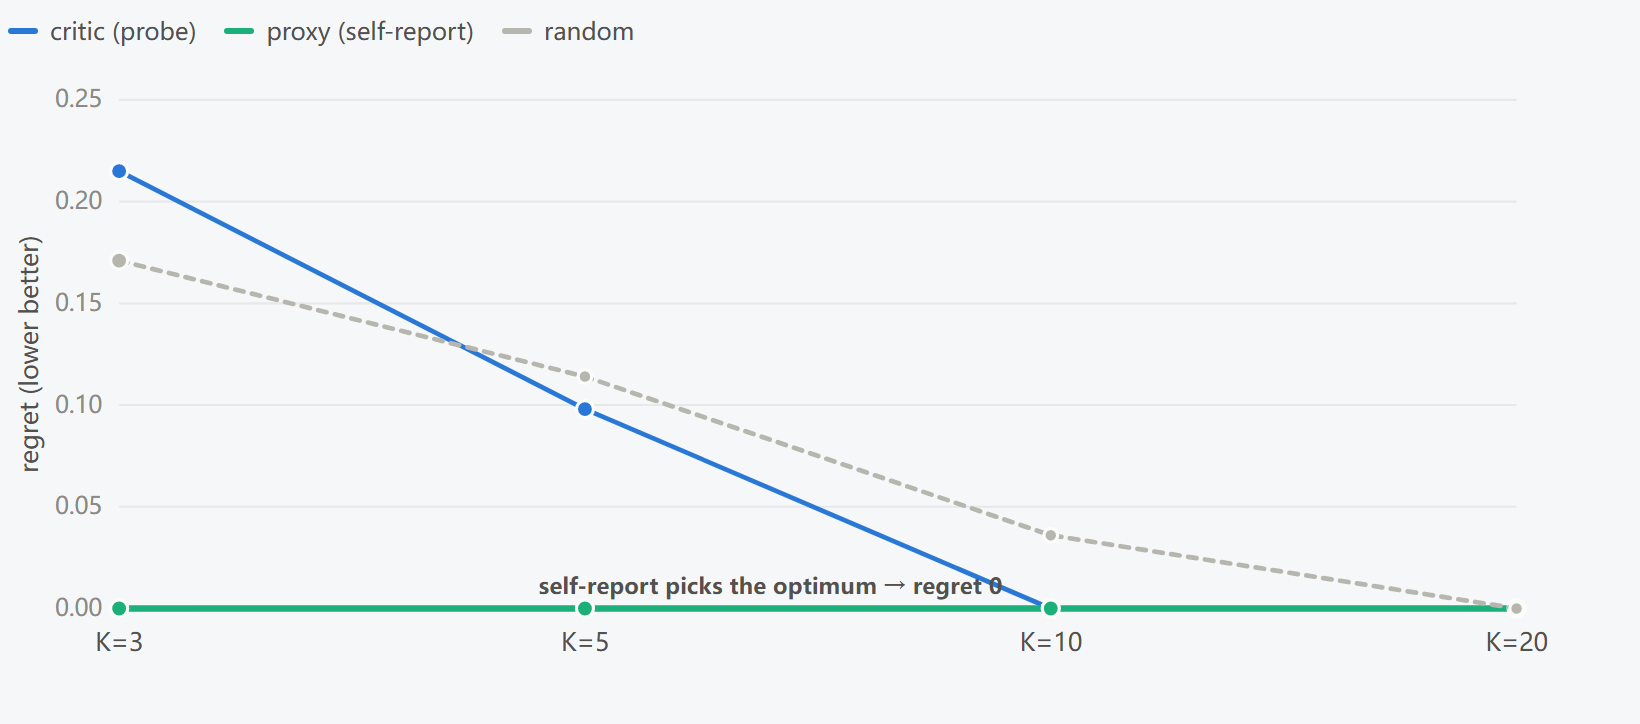
\includegraphics[width=\linewidth]{fig2.png}
\caption{\textbf{rank $\neq$ regret: the probe cannot save evaluations.} Best-of-$K$ under a budget of $K$: the free self-report proxy hits regret $0$; the probe is no better than random. Good rank (Fig.~\ref{fig:h1}) does not translate into savings.}
\label{fig:regret}
\end{figure}

\subsection{A deployment veto does not convert on real trees}
We wired the failure signal (\S\ref{sec:detect}) into deployment \textbf{as a veto}---override the self-report's pick when the probe distrusts it---and ran it offline first. \textbf{On random candidate pools it looks like a large win} ($\Delta$regret up to ${+}0.181$ at $K{=}20$ on spaceship; a soft blend $\arg\max\!\big(z(\text{self-report}){+}\lambda\,z(\text{probe})\big)$ cuts spaceship regret $0.235{\to}0.040$). \textbf{On real search trees it vanishes}: with each pool taken from one real spaceship run (18 runs, leave-one-run-out probe, no within-run leakage), a hard veto gives $\Delta$regret $\mathbf{-0.001}$ (3 win / 4 lose / 11 tie); the best soft blend gives ${+}0.007$ with 95\% bootstrap CI $[-0.003,+0.018]$---\textbf{not significant}. The random-pool win is an artifact of \emph{independent} candidates; real trees converge via improve-lineage, so the self-report's own pick is already good. \emph{rank $\neq$ regret} extends from best-of-$K$ selection to the online veto.

\subsection{The direction cannot be steered}
Decodability fails usability in a third, causal sense (Fig.~\ref{fig:steer}). We activation-steer the frozen model's layer-21 residual stream along the grade direction (CAA-style, ${\pm}3\sigma$ in units of its own projection std) and read the model's own soft score (expected value over the score digit's token distribution---a continuous readout, since the greedy score quantises to 7 buckets and is itself anti-correlated with the grade, \rhov{} $-0.21$). The quality-specific effect is \emph{statistically} detectable at $n{=}289$ but \textbf{negligible} (quality $-$ random slope ${+}1{\times}10^{-4}$, ${\sim}0.01\%$ of range), and a norm-matched \textbf{random} direction is itself ``significant'' (a generic perturbation)---the significance bar is meaningless at this power. The one direction that genuinely moves the output is \textbf{code length} (${\approx}4.5{\times}$ larger): the only steerable axis is a surface feature, exactly as steering-code work reports~\cite{steer}. So the \S\ref{sec:h1} grade signal is \textbf{decodable but not causally usable}---it selects nothing, vetoes nothing, and steers nothing; only surface features steer.

\begin{figure}[t]\centering
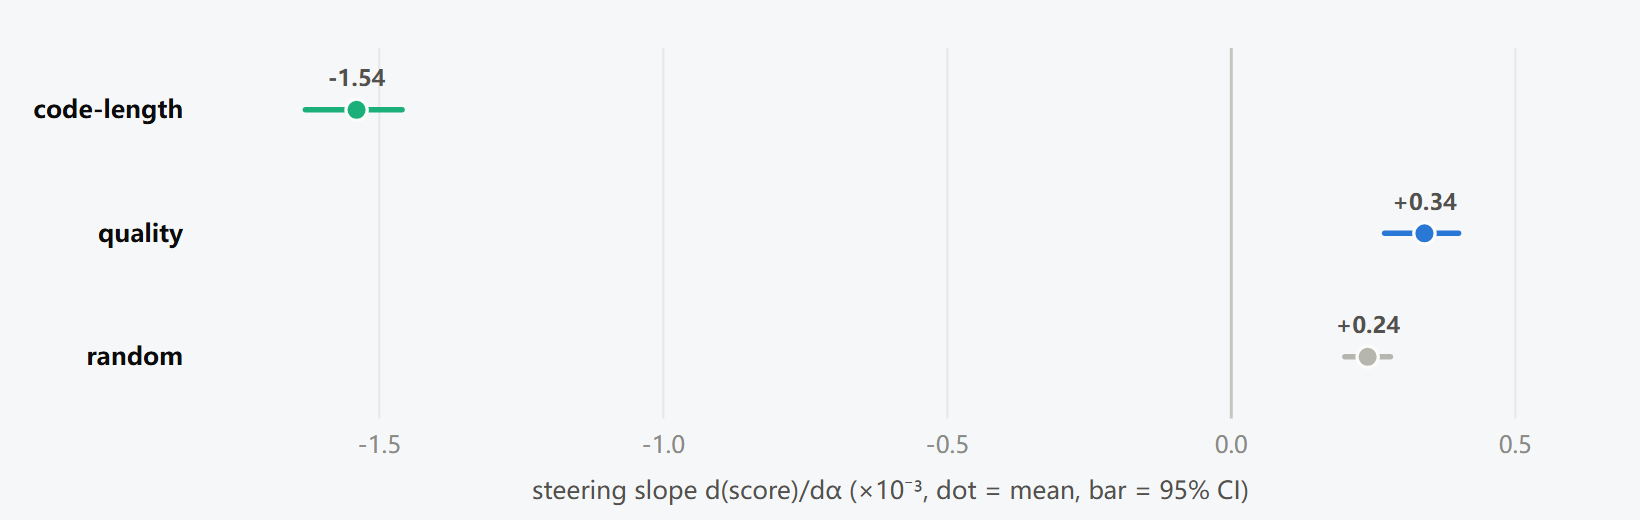
\includegraphics[width=\linewidth]{fig5.png}
\caption{\textbf{A3: the grade direction does not steer.} Steering slope of the model's soft score per direction ($\pm$95\% CI). The quality effect is negligible and barely above a random direction (itself ``significant''); only code length---a surface feature---moves the output.}
\label{fig:steer}
\end{figure}

\section{The one deployable use: failure detection}\label{sec:detect}
Where the probe earns its keep is where the self-report is \textbf{wrong}. On candidate pairs the self-report ranks incorrectly (0\% correct by construction; random 50\%), the probe is still right (Fig.~\ref{fig:rescue}): \textbf{0.59 on spaceship} (8{,}382 pairs), 0.55 nomad, 0.28 tps-may---a self-report-failure / reward-hacking detector, not a selector. Caveats: independence is \emph{partial} (0.59 $<$ probe-@-right 0.71) and \emph{not universal} (tps).

\begin{figure}[t]\centering
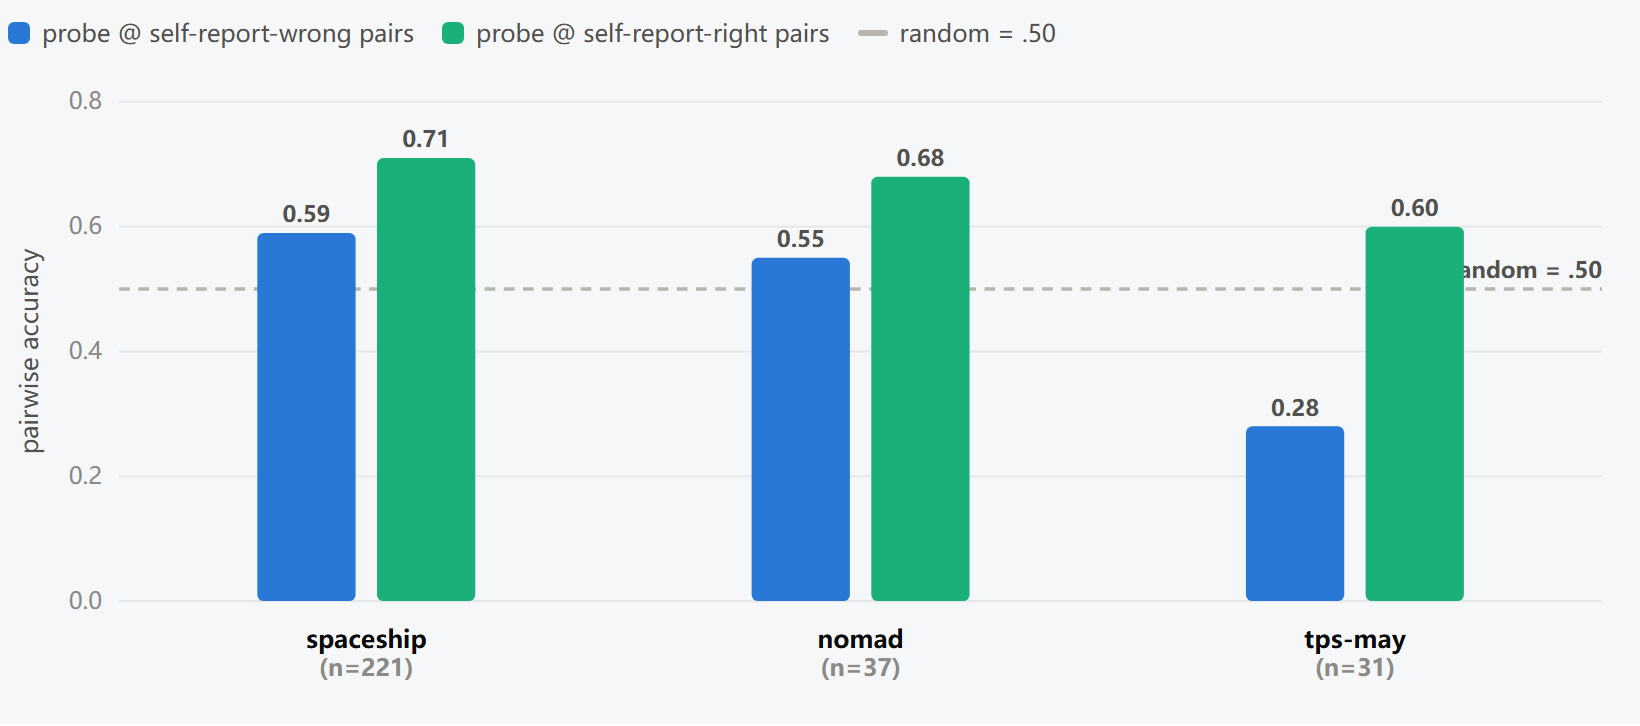
\includegraphics[width=\linewidth]{fig3.png}
\caption{\textbf{Rescue: the probe's value is where the self-report is wrong.} On pairs the self-report ranks wrong (random ${=}0.50$), the probe is still right ($0.59$ on spaceship). A failure detector, not a selector.}
\label{fig:rescue}
\end{figure}

\textbf{Made deployable, it beats the self-report and is not a length artifact---but it is modest.} As a per-candidate detector: among candidates the self-report already calls good (self-report ${\geq}$ its task median), flag the ones a \textbf{code-only} probe scores low. Pooled (146 such candidates, 38 secretly-below-median), the probe reaches \textbf{AUROC 0.63} $[95\%$ bootstrap CI $0.53$--$0.73]$ while the self-report's own score is \textbf{anti-informative} ($0.42 < 0.5$)---inside the set it already trusts, higher self-confidence is if anything a \emph{worse} signal, the sharpest form of ``the self-report cannot police itself''. The signal is \textbf{not code length}: residualising log-length out of the features per fold leaves AUROC unchanged ($0.62{\to}0.63$; length's marginal contribution $-0.01$ $[-0.07,+0.04]$). Limits stated plainly: the AUROC is \textbf{modest and statistically tied with a code-length heuristic} ($0.55$; the gap CI includes $0$, and fusing them adds nothing), and it is \textbf{spaceship-dominated} (nomad $n{=}5$ is uninformative). We report this as a downstream \emph{use} of the H1 signal~\cite{rh1,rh2,goodhart}, not a strong standalone detector.

\section{Two more non-levers}\label{sec:other}
\textbf{Reasoning-first does not help.} A reasoning-generation critic (analyse, then score) underperforms a scalar head overall (mean Spearman $-0.15$ vs $-0.07$). Teacher quality is a genuine hidden variable---a 7B$\to$14B teacher flips spaceship from $-0.01$ to $+0.31$---so a weak-teacher dismissal would be invalid; but the 14B gain does not generalise. We also tested the natural fix: give the teacher the \emph{true grade} so it writes a coherent rationale (privileged-information / hindsight), then distil. The rationales do become coherent, but on 231 labels the student \textbf{underfits}---default QLoRA collapses to the base model's zero-shot behaviour (byte-identical predictions); only aggressive training moves it off the base, and \emph{then} grounding helps by ${+}0.047$ (directionally validating the idea) yet the reasoning critic stays ${\sim}0.48$ below the scalar readout. Under poor compute a \textbf{frozen readout beats a trained reasoning critic}, precisely because it needs no expensive, underfitting generation training.

\textbf{Multi-fidelity has no headroom in the affordable regime.} From a candidate pool and a budget of $B$ full-eval-equivalents, \code{single} $=$ best of $B$ random, \code{mf(self-report)} $=$ best of the top-$B$ by the free self-report screen, \code{oracle} $=$ pool max. Headroom (\code{mf} $-$ \code{single}) is ${+}0.015$ (spaceship $B{=}3$), $-0.000$ ($B{=}10$), ${+}0.000$ (nomad), ${+}0.044$ (tps): essentially nil where evaluation is already affordable. The screen you would build is the free self-report, which \S5.1 already showed is a fine selector.

\section{Two methodological pitfalls}\label{sec:pitfalls}
\textbf{Prompt-truncation bug.} Code placed \emph{before} the instruction block in a length-limited prompt: truncation dropped the ``analyse-then-score'' instruction, the model \emph{continued the code}, and the parser grabbed a random number---the reasoning critic \emph{never ran} for a whole phase, invisible from metrics alone.
\textbf{Code-length confound.} Shortening code to fit a critic's VRAM \textbf{collapsed the probe's ablated Spearman from ${+}0.41$ to ${+}0.02$}---the probe reads the code. A confound in one arm silently inverted another arm's headline. (A sibling appears in \S\ref{sec:notusable}: a ``significant'' but negligible steering effect, tripped by over-powered statistics on a dead readout---always read the effect size and the random control, not the $p$-value.)

\section{Limitations}
Three tabular tasks, spaceship-dominated (221 / 37 / 31 cards); the per-task CIs on nomad and tps are wide, and we say so rather than average them away. The signal-is-there result is strong and cross-family; the not-usable and detection results are load-bearing on spaceship. Broadening to more (small) tasks is the natural next step but hits the compute wall that motivates the study---generating graded cards is itself expensive and must stay inside the fair contract. Everything here is a \emph{frozen-critic} result; it does not speak to fine-tuning the base, which the model-agnostic premise excludes by design.

\section{Conclusion}
A frozen code-LLM's representation \textbf{knows} more about an ML solution's eventual quality than the solution's own cheap self-report---decodably, independently of code length, low-dimensionally, and across model families. And it \textbf{cannot use} that knowledge to guide search under poor compute: it saves no evaluations, its deployment veto does not convert, and its quality direction cannot be steered; a trained reasoning critic and multi-fidelity screening add nothing. The one thing it buys is a length-independent flag for the failures the self-report hides. The practical reading is the one AIRA\_2 points to and we make single-GPU and model-agnostic: \textbf{the lever is clean, consistent evaluation, not a cleverer critic}---and the contribution is as much the set of cheap, adversarial, offline tests that \emph{separate a real signal from a usable one} as any single number.

\begin{thebibliography}{99}\small
\bibitem{airadojo} aira-dojo. arXiv:2507.02554.
\bibitem{aira2} AIRA\_2: high-consistency evaluation. arXiv:2603.26499.
\bibitem{elhsr} Mining Intrinsic Rewards from LLM Hidden States (ELHSR). arXiv:2505.12225.
\bibitem{openia} OPENIA. arXiv:2501.12934.
\bibitem{autoprobe} AutoProbe. arXiv:2510.02934.
\bibitem{ranker} Contrastive-direction code ranker. arXiv:2512.07404.
\bibitem{manifold} The Confidence Manifold. arXiv:2602.08159.
\bibitem{steer} Steering Code LLMs. arXiv:2603.23629.
\bibitem{rh1} Reward-hacking detection benchmark. arXiv:2601.20103.
\bibitem{rh2} Representation-level reward-hacking signals. arXiv:2604.01476.
\bibitem{goodhart} Goodhart's law / reward gaming. arXiv:2210.10760.
\bibitem{lengtharti} On surface/length artifacts in linear probes. arXiv:2606.02907.
\end{thebibliography}

\end{document}
